I've been within the fandom for about eleven years now, and only
relatively recently (about a year ago as of this post) did I get into
fursuiting. ~Prior to that, I must admit that I didn't understand the
concept at all, and even found it vaguely creepy. ~While I understood
the desire to more physically look like your character, I didn't
understand how fursuiting would be the solution: it seemed like wearing
a onesie of faux fur combined with slippers, gloves, and a ski-mask
coated in fur-covered foam was rather more like some elaborate Halloween
costume effect than getting nearer to one's character. ~However, having
gone suiting and wound up with a fursuit of my own, I think I'm gaining
a better understanding of it now.

Fursuiting is clinal, a gradient from one end of the spectrum to the
other. ~It can be very meaningful, where putting on the suit makes the
wearer into their character, or as close as possible. Or it can be
relatively meaningless, where suiting is closer to a job than anything,
something you do rather than something you are. ~Along the way, the
amount of meaning passes through the still very meaningful desire to at
least look like one's character, to enjoying the act of costuming
itself, to enjoying the varied social interaction that comes with
wearing a full-body costume somewhere other than Halloween.

As I grew within the furry subculture, I started out thinking that
everyone with a suit must be attempting to be their character in real
life, rather than just online. ~My opinion of how I would react to
suiting, however, was closer to the other end of the spectrum - I could
see how it might be fun to do that, but didn't really see it going
further, for myself. ~As time went on, though, I started to experience
how suiting was different for different people, and, at the same time, I
felt myself climbing the scale in the opposite direction. ~The concept
started to make more sense to me, and I could understand how someone
might enjoy looking rather more like an animal, specifically like their
character, even if it was most definitely in the context of costuming.
~Sometime in 2010, these two converging lines met when I was given the
opportunity to try a friend's suit for a day at Anthrocon.

\begin{figure}[htbp]
\centering
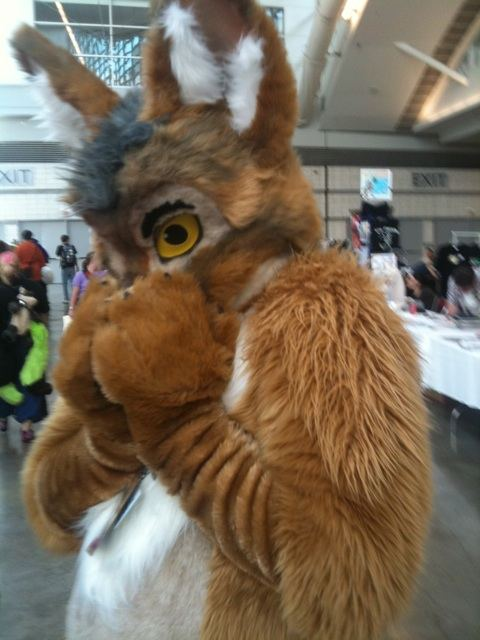
\includegraphics{http://adjectivespecies.com/wp-content/uploads/2011/12/1277784733.ranna_2i6r.jpg}
\caption{One Gay Jackal}
\end{figure}

The friend is a bit of a sarcastic sort, and he had a black-backed
jackal suit that I wanted to try on to see if I could (jokingly) sully
his reputation by acting super furry and overtly homosexual. ~It just so
happened that we were the right size and he thought it was as good an
idea as I did, so I went up to his room at ten or so in the morning and
put on the suit. ~I was immediately surprised by how warm it was, and I
had a bit of a hard time getting used to it, at first, since Pittsburgh
in the summer is already plenty warm. ~It was a bit of a trial getting
from the convention hotel to the convention center, though it's a
relatively short walk. ~Once I got inside, however, I really started to
get into the swing of things.

I had a lot of fun interacting with people around me. ~A surprising
amount of fun, really. ~I was expecting that, wearing a full body
costume that required a wicking layer, I'd be uncomfortable, but goof
around and act flamingly gay for a little while, then head back to the
room to strip it off. ~However, the costume was comfortable and I felt
comfortable acting like a fool in it. ~Wearing paws and having a stuffed
tail behind me made me walk different just to see how it felt, and those
around me ate up the fact that I was a big dog-man acting like a nutjob.
~I wore the suit longer than intended; I made a few stops by the
``headless lounge'', ambled around the dealer's den, followed people
around and mimicked them, and spent more time than I usually would
talking to, playing with, and otherwise just interacting with furries.
~When I got home, I placed an order with the maker of the fursuit, Jill
of jillcostumes for my own, settling on an otter after some discussion.

\begin{figure}[htbp]
\centering
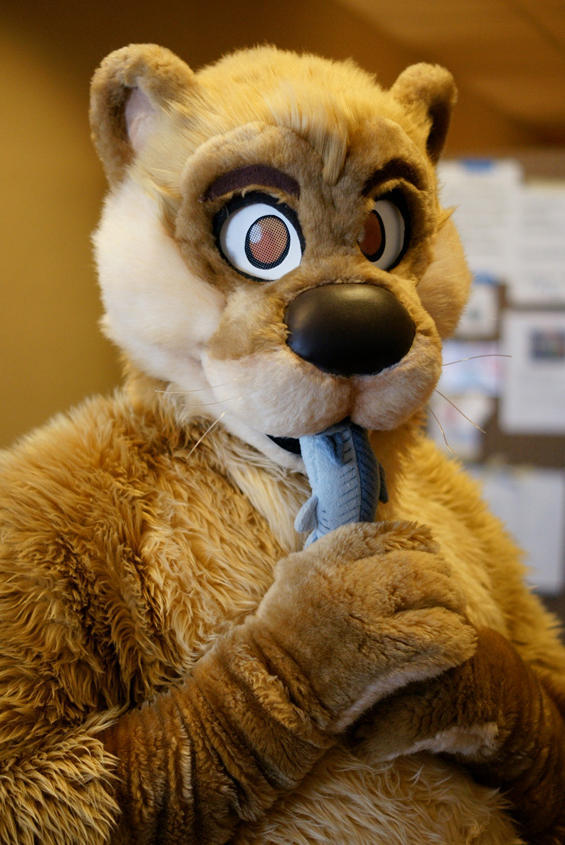
\includegraphics{http://adjectivespecies.com/wp-content/uploads/2011/12/1313468502.ranna_rocky-mountain-fur-con-2011.7113233.87.jpg}
\caption{A member of the otter-man empire}
\end{figure}

That was about the time I started to realize the diversity apparent
within a subculture of a subculture. ~There was more, I figured, to
wearing a fursuit than just getting closer to your character, being your
avatar. ~It was a whole different way of interacting with those around
you, whether you're one of those suiters that never talks or one that
rambles on in suit (I am, of course, the latter). ~Having asked, there
are those who do feel like it brings out aspects of their personality
that bring themselves closer to their character, but that's not the only
way of looking at it out there: there are those who find them sexually
attractive, those that like them because of the social interaction with
those who aren't necessarily part of the fandom (interacting with kids
is mentioned as being particularly awesome), and those for whom it is a
living. ~It's a whole spectrum, just as are other aspects of furry, but
it comes with its own culture: listen in on conversations in a headless
lounge and they're most certainly unique.

Things aren't all sunshine and roses, of course. ~One of the first
things I found out once I got my suit was how to clean it, and how
divisive such an act was. ~There are currents and trends of thought
within the suiting culture just as there are within furry as a whole,
and something as simple as washing a portion of your suit can cause
strife. ~Having personally known the maker of my suit, I trusted her
when she gave me instructions for washing not only the bodysuit but also
the head in the washing machine. ~However, even after she posted a video
of how she cleans her own and her customer's fursuit heads without harm,
others within the fandom insisted that she was damaging the heads that
she had made, despite all evidence pointing to the contrary. ~Similar
discussions rage around how best to transport your suit from place to
place, particularly on a plane. ~Any fursuit lounge is bound to be
filled nearly to the brim with Rubbermaid Action Packers, while anyone
(say, yours truly) who travels with his suit in a duffel is scoffed at
openly.

And then there are the people. ~Oh, the people. ~Not every interaction
is a positive one. ~In fact, we can start to break down the other
parties into rough categories:

\begin{itemize}
\tightlist
\item
  \textbf{The Talker}~- The talker will hover close, and may or may not
  be affectionate, but will insist on talking to you ``out of
  character''. ~Rather than interacting with a fursuiter, they will
  insist on interacting with a person wearing a costume. ~``This is
  really well made!'', they will say. ~``I think this is a cute one, but
  the older version was cuter, in my mind,'' you will be informed.
  ~``One doesn't see black-backed jackals all that much, it's nice to
  see that the colors are very accurate,'' they'll say, pointing out the
  patterning on the suit despite your lack of peripheral vision. ~The
  talker is mostly harmless. ~Mostly. ~You can't spell `stalker' without
  it, though, and it's only a few minutes too long of following you
  around that separates the two.
\item
  \textbf{The Toucher}~- This is the one we all kind of worry about.
  ~You'll be wandering around, and someone (99.44\% chance that they're
  male) will open their arms for a hug. ~``Sure!'' you think/mime/say
  and approach them. ~They'll hug you and maybe coo at how cute your
  suit is. ~And the hug will linger. ~And go on a little too long. ~And
  you'll try to pull away, and the Toucher will laugh and ruffle his
  hands down over your back, sides, or front, and then it will come: the
  Touch. ~Sometimes the touch is fumbling and quick, because you're
  likely in public, but it's even worse when it's not, the Toucher
  grabbing rather firmly at some decidedly tender bits or giving your
  backside a squeeze. ~The worst part about this, for me, is that all I
  feel I can do is just get away. ~It's surprisingly hard to tell
  someone to stop or to move their hand when you're dressed as a giant
  otter.
\item
  \textbf{The Maker}~- The Maker is closely related to the Talker and
  the Toucher, though obviously more innocent than either. ~They will
  spend a lot of time touching you while talking out of character. ~The
  whole time, though, rather than grabbing at your crotch, they're
  feeling along the seams of your suit or inspecting the eyes'
  construction, all while talking about air-brushing or fur selection.
  ~While not quite as offensive as the Talker or the Toucher, this is
  nonetheless still quite awkward for someone who most certainly did not
  make their own suit.
\item
  \textbf{The Fursuit Hater}~- I don't know what to do about it. ~Look,
  I'm sorry that I'm a grown-ass man dressed as a giant otter among a
  bunch of other grown-ass men. ~I'm having fun, others are having fun,
  and those that aren't are doing something else. ~Why do you need to
  tell me that fursuits are creepy and probably gross and covered in
  semen and \emph{countless other things I really don't care to hear
  about}. ~You pretend to be an animal-person, too.
\item
  \textbf{The Other Suiter}~- This one's up in the air. ~Normally,
  hanging around other fursuiters while in suit is pretty awesome. ~You
  can commiserate about those around you, play around and get some
  laughs (and plenty of pictures), and just plain have fun.
  ~Occasionally, though, you'll run into a suiter that also happens to
  be a Toucher, or even more so. ~I don't deny that some suits are
  pretty attractive, of course; the problem lies more in the lack of
  respect for differing opinions, especially around how to act in a
  public place. ~Fursuits serve to offer some of the same anonymity
  provided by the internet, and there has been more than once instance
  of someone grabbing or grinding on me in a scratchy, hot, faux-fur
  onesie in a hallway or dance that has led to quite a bit of
  discomfort.
\end{itemize}

\begin{figure}[htbp]
\centering
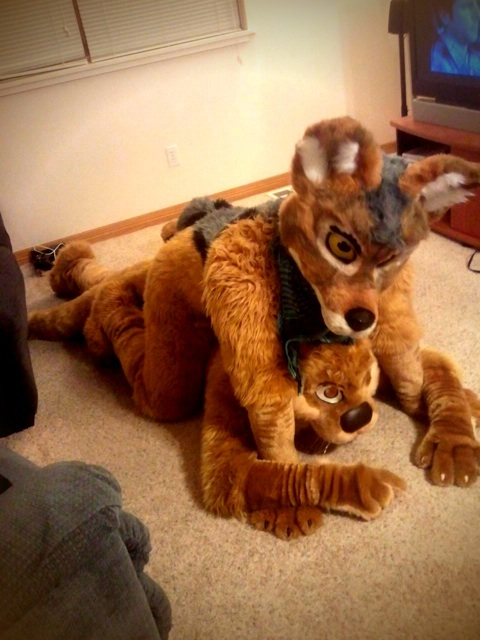
\includegraphics{http://adjectivespecies.com/wp-content/uploads/2011/12/1296050316.ranna_5nqb.jpg}
\caption{Repayment for borrowing the suit}
\end{figure}

Even with the occasional bad apple, it's definitely more fun than not to
pretend to be an animal person, or at least interact as one, or to act a
fool as one. ~I picked up my suit at Further Confusion 2010 from Jill
once I arrived at the hotel. ~Just for giggles, I wore the suit as a
partial for the rest of the night, roaming around to find people I knew
so as to surprise them. ~I stole sips of beer, batted at people with my
paws, poked my enormous nose on them, and basically just had fun. ~It's
another way to entwine yourself with this strange fandom of ours, and
provides a unique mixture of in- and out-of-character interactions with
those around you. ~For some, it's a way to become their avatar, and for
others it's a fun way to, in the jackal's words, ``get drunk and touch
friends.'' ~And, whether you're a fan of them or not, suiters are an
integral part of our subculture, shaping not only our own interactions
but the views of those looking in from outside.
